\documentclass[varwidth=\maxdimen]{standalone}
\usepackage{tikz}
\usetikzlibrary{fit}
\usepackage[nomessages]{fp}

\tikzset{every label/.style={font=\footnotesize,inner sep=1.5pt}}

\newcommand{\pc}[4][]{\node[circle, fill, label={below:#4},#1] at (#2) (#3) {}}
\newcommand{\pcghost}[4][]{\node[circle, fill=gray, label={below:#4},#1] at (#2) (#3) {}}
\newcommand{\pu}[4][]{\node[rectangle, fill=blue, label={above:#4},#1] at (#2) (#3) {}}
\newcommand{\pughost}[4][]{\node[rectangle, fill=gray, label={above:#4},#1] at (#2) (#3) {}}
\newcommand{\nx}{4} %number of cells in x direction
\newcommand{\nghost}{2} %number of ghost cells in x direction
\newcommand{\xmin}{0}  %grid start
\newcommand{\xmax}{12} %grid end

\begin{document}
	\begin{figure}[h]
		\centering
		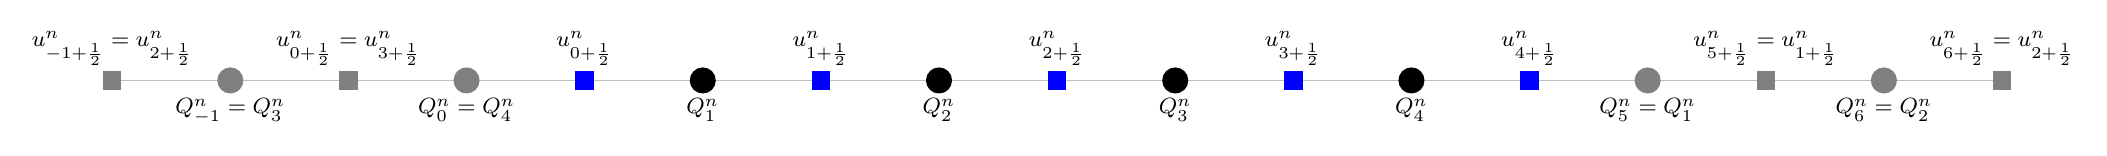
\begin{tikzpicture}
			% Grid lines
			\FPeval{\dx}{clip((\xmax-\xmin)/\nx)}
			\draw[gray!50, thin] (\xmin -\nghost*\dx,0) -- (\xmax+\nghost*\dx,0);
			
			% Interior grid centers
			\foreach \i in {1,...,\nx}{
				\FPeval{\xc}{clip(\xmin+(\i-0.5)*\dx)}
				\pc{\xc,0}{5}{$Q_{\i}^n$};
			}
			
			% Ghost cell centers
			\foreach \i in {1,...,\nghost}{
				\FPeval{\xc}{clip(\xmin-(\nghost-\i+0.5)*\dx)}
				\FPeval{\ii}{clip(\i-\nghost)}
				\FPeval{\iii}{clip(\nx+\ii)}
				\pcghost{\xc,0}{5}{$Q_{\ii}^n=Q_{\iii}^n$};

				\FPeval{\xc}{clip(\xmax+(\i-0.5)*\dx)}
				\FPeval{\ii}{clip(\nx+\i)}
				\FPeval{\iii}{clip(\i)}
				\pcghost{\xc,0}{5}{$Q_{\ii}^n=Q_{\iii}^n$};
			}
			
			% Interior grid edges
			\foreach \i in {0,...,\nx}{
				\FPeval{\xc}{clip(\xmin+\i*\dx)}
				\pu{\xc,0}{5}{$u_{\i+\frac{1}{2}}^n$};
			}
			% Ghost cell edges
			\foreach \i in {1,...,\nghost}{					
				\FPeval{\xc}{clip(\xmax+\i*\dx)}
				\FPeval{\ii}{clip(\nx+\i)}
				\FPeval{\iii}{clip(\i)}
				\pughost{\xc,0}{5}{$u_{\ii+\frac{1}{2}}^n = u_{\iii+\frac{1}{2}}^n$};

				\FPeval{\xc}{clip(\xmin-(\nghost-\i+1)*\dx)}
				\FPeval{\ii}{clip(\i-\nghost)}
				\FPeval{\iii}{clip(\nx+\ii-1)}
				\pughost{\xc,0}{5}{$u_{\ii+\frac{1}{2}}^n = u_{\iii+\frac{1}{2}}^n$};
			}
		\end{tikzpicture}
	\end{figure}
\end{document}
